\documentclass[12pt, a4paper]{article}

% Font & text
\usepackage{times}
\usepackage[utf8]{inputenc} 
\setlength{\parindent}{0in}
\usepackage{hyperref}
\hypersetup{%
    pdfborder = {0 0 0}
}
\usepackage{caption}
\usepackage{subcaption}
\usepackage{float}

% Math
\usepackage{amsmath}
\usepackage{amssymb}
\usepackage{mathtools}

\newcommand{\im}{\mathrm{Im}}
\newcommand{\p}[1]{\left( #1 \right)}
\newcommand{\lr}[3]{\left#1 #3 \right#2}
\newcommand{\st}{\mathrm{s.t.}}
\newcommand{\N}{\mathbb{N}}
\newcommand{\Z}{\mathbb{Z}}
\newcommand{\B}{\mathbb{B}}
\newcommand{\R}{\mathbb{R}}
\newcommand{\atan}{\mathrm{atan}}
\newcommand{\atantwo}{\mathrm{atan2}}
\newcommand{\Oh}{\mathcal{O}}
\newcommand{\lineseg}[1]{\overline{#1}}

% Source code
\usepackage{listings}
\usepackage{color}

\newcommand{\addcode}[1]{
\subsection*{#1}
\lstinputlisting[language=python, xleftmargin=-5em,xrightmargin=-5em]{../#1}
}

\lstset{
    language=Python,
    showstringspaces=false,
    breaklines=true,
    breakatwhitespace=false,
    formfeed=\newpage,
    tabsize=4,
    numbers=left,
    numbersep=5pt,
    numberstyle=\tiny\color{gray},
    commentstyle=\itshape\color{gray},
    keywordstyle=\bfseries\color{blue!40!black},
    identifierstyle=\color{black},
    stringstyle=\color{green!50!black},
    basicstyle=\ttfamily,
    morekeywords={lambda}
}


% Algorithms
\usepackage[noend]{algpseudocode}
\usepackage{algorithm}

\makeatletter
\def\BState{\State\hskip-\ALG@thistlm}
\makeatother


% Proofs
\usepackage{amsthm}

\newtheorem{theorem}{Theorem}[section]
\newtheorem{corollary}{Corollary}[theorem]
\newtheorem{lemma}[theorem]{Lemma}

\renewcommand\qedsymbol{$\blacksquare$}


% Page, Header & Footer
%\usepackage{geometry}
\pagestyle{empty}
\usepackage{lastpage}
\usepackage{fancyhdr}
\pagestyle{fancy}
\fancyhead{}
\fancyhf{}
\renewcommand{\headrulewidth}{0pt}
\cfoot{}
\rfoot{\thepage\ of \pageref{LastPage}}
\rhead{}

% Images
\usepackage{tikz}

\usepackage{titling}
\date{26th October 2016}
\author{Jon Kingo Christensen}
\def\identification{Jon Kingo Christensen, 180491, jonch10@student.sdu.dk}
\def\courseCode{DM803}
\def\courseTitle{Advanced Datastructures}
\def\lectorLabel{Teacher:}
\def\lector{Kim Skak Larsen}
\def\universityName{Syddansk Universitet}
\def\papertitle{Assignment 1}
\def\papersubtitle{\courseTitle}
\title{\papertitle{} - \papersubtitle{}}




% ============ %
\begin{document}
%\maketitle

\begin{tabular}{@{}l}
\universityName{} \\
\lectorLabel{} \lector{}
\end{tabular}
\hfill
\begin{tabular}{r@{}}
\courseTitle{} (\courseCode{}) \\
\thedate{}
\end{tabular}

\bigskip

% Frontpage Title
\begin{center}
    \Huge{\papertitle{}} \\
    \Large{\papersubtitle{}}
\end{center}
\normalsize{}

\begin{center}
    \identification{}
\end{center}

%\bigskip

%\newpage

%\restoregeometry{}



\section*{Specification}
This report describes the implementation of random trees as specified in the
assignment,
and partially persistent linked lists in the programming language python.


\section*{Formatting details}
The datastructures have been implemented in python version 3.4.3 and this is the version that should be run for testing it.
On the IMADA terminal machines this is done using python3.

\medskip

The programs read from \texttt{stdin} and writes to \texttt{stdout}, an example of running the random tree using an input file and writing
to an output file can be seen below:
\begin{lstlisting}[language=bash]
  python3 randomTree.py < inputfile > outputfile
\end{lstlisting}

\section*{Random Trees}
Random trees is a mix between a search tree and a heap, but where
nodes in the random tree have uniformly random priorities assigned.

\subsection*{Input/Output}
Input for random trees is a number of lines each consisting of one capital 
letter, possibly followed by one space and then some symbol.
The letters and their meaning are as follows: 
"I" followed by a key will insert said key into the tree.
"D" followed by a key will delete said key from the tree.
"S" followed by a key will search for said key in the tree.
"M" followed by a key will first split the tree with said key as split value,
and then merge the two resulting trees. The key can't already exist in the tree.
"T" followed by a "D", will do a traversal of the 
tree and print all keys in the tree and their depth in the tree. and then 
the average depth of the tree. If it is followed by an "A" instead, it will only
print the average.

\medskip
Output for random trees is dependent on the input, if an insertion, 
deletion, or search is successful
an "S" is printed, and if unsuccessful an "F" is printed. 
Merging will print an S if successful and if not it will print whether
a merge was attempted with an empty tree (a key with too 
large or small value given), or if the key given was already
in the tree.


\subsection*{Implementation}
The random tree is implemented as described in the assignment. 
The tree structure itself only has a pointer to the root.
The nodes only have information for children pointers, priority value 
and the key of the node.
Priorities are chosen at random (as uniformly random as python is able to do)
from all integers in the range $[1,2^30-1]$.
\textbf{Insert} is implemented using an ancestor list, so that the single
rotations to fix the priority structure does not need nodes to have parent pointers.
Then after inserting, The inserted node will make single rotations with
it's parent node as long as it has a parent with a smaller priority than itself.
It is not possible to insert duplicates
\textbf{Split} inserts a node with priority 0 (smaller than any other in tree)
so it becomes the root and then returns the two children of the node.
The split value given must be an integer not in the tree or the insert method will return false.
One could change it so that duplicates are allowed and split values could 
be present in the tree. It would just require the insert method to "search" left or right when hitting it's own value.
\textbf{Delete} Checks whether the two subtrees that are to be merged are empty. And handles each possible case (for example if left subtree is empty, just 
replace deleted node with right subtree). 
It also checks if the root was deleted and reassigns the trees root pointer to
the new root.
\textbf{Traverse} is a simple tree traversal where depth is updated underways
and also where the size of the tree and the sum of all depths are counted. 
This is to find the average depth as well. 


\subsection*{Testing}
The access time of nodes in a tree can be described as the depth of said node.
To find the depth of all node and to calculate the average, the method
{\it traverse} was written. It prints all node depths and also the average depth.

The program {\it maketest.py} was used to generate different kinds of input 
since it will be interesting to see how the random tree performs against 
different inputs.
\paragraph{Random input}

\paragraph{Sorted input}

\paragraph{Reversely sorted input}

%TODO: write about tests



\section*{Partially Persistent Linked Lists}
Input for Partially Persistent Linked Lists (PPLL) is a number of lines each
consisting of capital letters possibly followed by keys seperated by space.
The letters and their meaning are as follows: 
"I" followed by a key {\it k} will insert said key into the list in the 
newest version on the {\it k}th index.
"S" followed by a version number {\it v} and an integer {\it i} 
will return the {\it i}th element ofthe {\it v}th version of the list.
"U" followed by an key {\it k} and integer [\it i] will update the {\it i}th
element to have the key {\it k} in the newest version of the list.
"N" will change the list to a new version.
"V" will print what version number the newest version is.
"T" followed by a version number, will traverse and print all keys in the 
list of said version number.
"TA" will traverse all versions of the PPLL.

\medskip
As for the unmentioned output, inserting, updating, and changing version 
will print an "S" if it was successful
and an "F" if not. Search will print an "S" followed 
by the key in the node found
if successful and an "F" if unsuccessful. 

\subsection*{Implementation}
The PPLL is implemented using copy nodes, the idea is that when a node goes 
through changes, either through updates or updates of pointers. Newer versions 
of the node can be represented by a copy of the node, and then updating pointers
makes sure that you find the correct version of the node you want when you need it.
The PPLL itself holds a header list, a version number to keep track of the newest version,
and a variable e, to determine the number of extra pointers allowed in a node.
A node has its key, and next and previous pointer, a version number, and a list of
extra pointers.
%TODO: And possibly a copy pointer???
The implementation of PPLL was simplified using some utility methods, 
using these as blackboxes simplifies the readability of the code as well as the
pseudocode. They are as following:
\paragraph{newestNext(x,v)} finds the newest next pointer of node x 
which still has a version older than or equal to v.
\paragraph{newestPrev(x,v)} like newestNext but with previous pointer instead. 
\paragraph{makecopy(original, isleft, a)} makes a copy of the {\it original} node.
It is assumed that the node [\it a} is the node which is the reason for having to 
make a copy of {\it original}, and {\it isleft} is a boolean value indicating if
{\it original} is a previous node of a.
if {\it isleft} is true, makecopy, makes a copy of {\it original} using {\it a}
as the next pointer, and sets the previous pointer to the newestPrev of 
{\it original}. The next pointer of whatever said previous pointer points to,
must then also be updated. And if there's no room for such a new pointer. 
Then a copy must also be made of this node recursively. 
If isleft is false, then it's the same, but with next and prev reversed.
\paragraph{pointerUpdate(y)} updates the node {\it y} so it has correct pointers, 
and so pointers point to it correctly. It assumes that the node {\it y} already
has its pointers set, so they only need to be updated, if copy nodes are made.
The method goes through neighboor nodes and adds pointers to {\it y}, unless
there already exists pointers of {\it y}'s version, then they are overwritten.
If there are not room in the extra list for new pointers, then a copy node is 
made using the {\it makecopy} method. If {\it y} is the first element of the 
list, then a pointer is added to the headerlist of the PPLL.

\medskip
Search is implemented by following the newest pointer in a node still older 
than or same version as the version that is being searched in. This is done until 
the i'th element is found. The pseudocode for search can be seen in Algorithm \ref{search}.

\begin{algorithm}
\caption{Search}\label{search}
\begin{algorithmic}[1]
\Procedure{Search}{$v,i$}
    \If{header is empty}
        \State return None
    \EndIf
    \State $x \gets $ newest node in header, older than v. 
    \While{$i > 1$}
        \State $x \gets newestNext(x,v)$
        \If{x is None}
            \State return x
        \EndIf
        \State $i \gets i-1$
    \EndWhile
    \State return x
\EndProcedure
\end{algorithmic}
\end{algorithm}

\medskip
Insert is done by finding the point of insertion. Then from the inserted 
nodes perspective, inserting it so the pointers are correct. Afterwards 
using the {\it pointerUpdate} method to make sure the surrounding nodes have 
correct pointers. The method also takes care of making copy nodes. The 
pseudocode for insertion can be seen in Algorithm \ref{insert}.

\begin{algorithm}
\caption{Insert}\label{insert}
\begin{algorithmic}[1]
\Procedure{Insert}{$k,i$}
    \State $y \gets$ new node with key $k$
    \If{$i == 1$}
        \State $y.next \gets$ newest first element
        \State $pointerUpdate(y)$
    \Else
        \State $y.prev \gets Search(newestVersion, i-1)$\Comment{newestVersion is the newest version as specified by the PPLL's version}
        \State $y.next \gets newestNext(y.prev, newestVersion)$
        \State $pointerUpdate(y)$
    \EndIf
    \State return True
\EndProcedure
\end{algorithmic}
\end{algorithm}

\medskip
Updating a node is done by finding said node, and if the node was created in
the same version, then just changing the key. Otherwise a copy node is created
with the new key. The copy node gets the most recent pointers of the original node
as its previous and next pointers. Afterwards the method {\it pointerUpdate} is used
to correct surrounding pointers and possibly create other copy nodes. 
The pseudocode for updating can be seen in Algorithm \ref{update}

\begin{algorithm}
\caption{Update}\label{update}
\begin{algorithmic}[1]
\Procedure{Update}{$k,i$}
    \State $x \gets Search(newestVersion, i)$
    \If{$x$ is None}
        \State return False
    \endIf
    \If{$x.version == newestVersion$}
        \State $x.key \gets k$
        \State return True
    \EndIf
    \State $copy \gets$ new node with key $k$
    \State $x.copy \gets copy$
    \State $copy.prev \gets newestPrev(x, newestVersion)$
    \State $copy.next \gets newestNext(x, newestVersion)$
    \State $pointerUpdate(copy)$
    \State return True
\EndProcedure
\end{algorithmic}
\end{algorithm}
%TODO:write about implementation

\subsection*{Testing}

%TODO: write about tests




%%%%%%%%%%%%%%%%%%%%%%%%%%%%%%%%%%%%%%%%%%%%%%%%%%%%%%%%%%%%%%%%%%%%%%%%
%%%%%%%%%%% FOLLOWING IS OLD STUFF AND SHOULD BE DELETED!!! %%%%%%%%%%%%
%%%%%%%%%%%%%%%%%%%%%%%%%%%%%%%%%%%%%%%%%%%%%%%%%%%%%%%%%%%%%%%%%%%%%%%%
\section*{Testing}
The program maketest.py has been written to generate examples for the tests given in this section. 
Specifically \texttt{test1} was used for the average search complexity.
To evaluate p values in skip lists, and variations in search complexity \texttt{test2} was used. 
And finally test3 and others were used to look at size and frequency of rebuilds in scapegoat trees.
The \texttt{manual.txt} document describes how to use this tool if the tests needs to be recreated.

\subsection*{Average search complexity}
The average search times have been investigated by repeatingly inserting 50 elements into the data structure, and then searching 50 times for some 
element in the datastructure (including previously added elements). Then taking the average of the comparisons used for each of the 50 searches.
Fig. \ref{avgsearch} shows the results of doing this up until 100.000 elements have been inserted.

\begin{figure}[H]
    \centering
    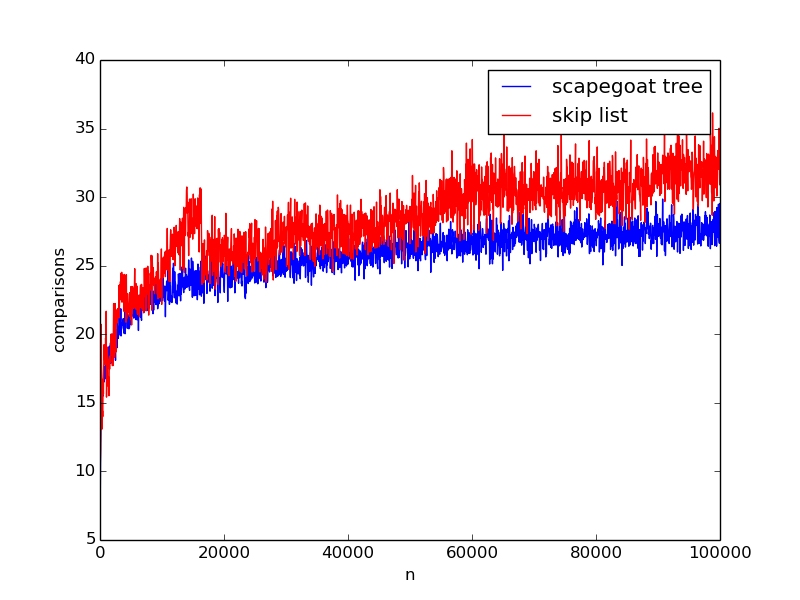
\includegraphics[width=1\textwidth]{averagesearch.png}
    \caption{scapegoat tree and skip list average search times.}
    \label{avgsearch}
\end{figure}


\medskip


The constants follow the same trend as in the article, where it first goes down, then starts growing again. although here it appears that the 
p value of a half is a bit better than that of a quater, unlike the article. The values are also generally larger than in the article.


\subsection*{Variation in search complexity}
The variation of the search complexity can be found by doing many searches and recording for each i, how many searches required i comparisons.
This has been evaluated by creating a random shuffle of 100.000 integers and inserting them. Then all the same integers are searched for.
This eliminates duplicate searches which is not as relevant here as getting the full spectrum of search complexities is. The results 
can be seen in Fig. \ref{variation}

\begin{figure}[H]
    \centering
    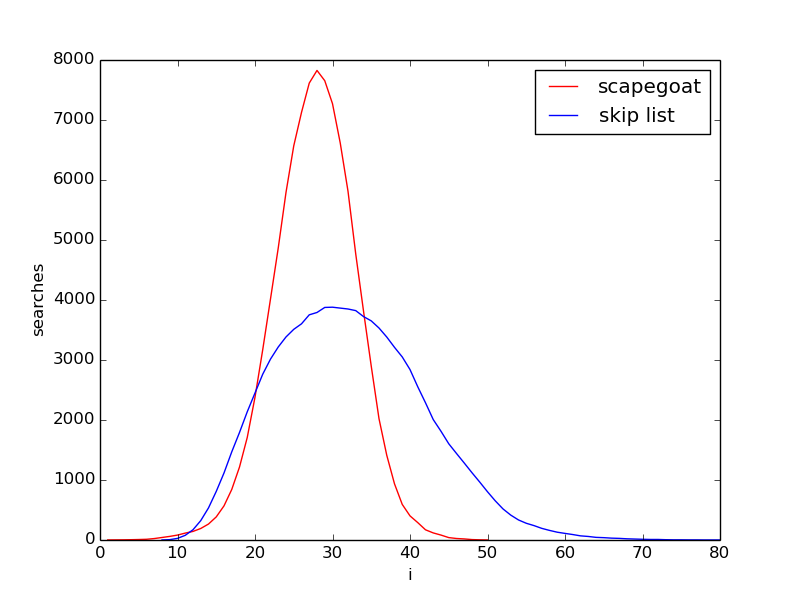
\includegraphics[width=1\textwidth]{variation.png}
    \caption{variation of search complexities for scapegoat trees and skip lists.}
    \label{variation}
\end{figure}

The graph shows that scapegoat trees has a more narrow variation, and it's generally a bit lower than skip lists.




\section*{Conclusion}

























\end{document}
